\documentclass[twoside]{book}

% Packages required by doxygen
\usepackage{fixltx2e}
\usepackage{calc}
\usepackage{doxygen}
\usepackage{graphicx}
\usepackage[utf8]{inputenc}
\usepackage{makeidx}
\usepackage{multicol}
\usepackage{multirow}
\PassOptionsToPackage{warn}{textcomp}
\usepackage{textcomp}
\usepackage[nointegrals]{wasysym}
\usepackage[table]{xcolor}

% Font selection
\usepackage[T1]{fontenc}
\usepackage{mathptmx}
\usepackage[scaled=.90]{helvet}
\usepackage{courier}
\usepackage{amssymb}
\usepackage{sectsty}
\renewcommand{\familydefault}{\sfdefault}
\allsectionsfont{%
  \fontseries{bc}\selectfont%
  \color{darkgray}%
}
\renewcommand{\DoxyLabelFont}{%
  \fontseries{bc}\selectfont%
  \color{darkgray}%
}
\newcommand{\+}{\discretionary{\mbox{\scriptsize$\hookleftarrow$}}{}{}}

% Page & text layout
\usepackage{geometry}
\geometry{%
  a4paper,%
  top=2.5cm,%
  bottom=2.5cm,%
  left=2.5cm,%
  right=2.5cm%
}
\tolerance=750
\hfuzz=15pt
\hbadness=750
\setlength{\emergencystretch}{15pt}
\setlength{\parindent}{0cm}
\setlength{\parskip}{0.2cm}
\makeatletter
\renewcommand{\paragraph}{%
  \@startsection{paragraph}{4}{0ex}{-1.0ex}{1.0ex}{%
    \normalfont\normalsize\bfseries\SS@parafont%
  }%
}
\renewcommand{\subparagraph}{%
  \@startsection{subparagraph}{5}{0ex}{-1.0ex}{1.0ex}{%
    \normalfont\normalsize\bfseries\SS@subparafont%
  }%
}
\makeatother

% Headers & footers
\usepackage{fancyhdr}
\pagestyle{fancyplain}
\fancyhead[LE]{\fancyplain{}{\bfseries\thepage}}
\fancyhead[CE]{\fancyplain{}{}}
\fancyhead[RE]{\fancyplain{}{\bfseries\leftmark}}
\fancyhead[LO]{\fancyplain{}{\bfseries\rightmark}}
\fancyhead[CO]{\fancyplain{}{}}
\fancyhead[RO]{\fancyplain{}{\bfseries\thepage}}
\fancyfoot[LE]{\fancyplain{}{}}
\fancyfoot[CE]{\fancyplain{}{}}
\fancyfoot[RE]{\fancyplain{}{\bfseries\scriptsize Generated on Sun Dec 7 2014 18\+:13\+:55 for Compound\+Data\+Types by Doxygen }}
\fancyfoot[LO]{\fancyplain{}{\bfseries\scriptsize Generated on Sun Dec 7 2014 18\+:13\+:55 for Compound\+Data\+Types by Doxygen }}
\fancyfoot[CO]{\fancyplain{}{}}
\fancyfoot[RO]{\fancyplain{}{}}
\renewcommand{\footrulewidth}{0.4pt}
\renewcommand{\chaptermark}[1]{%
  \markboth{#1}{}%
}
\renewcommand{\sectionmark}[1]{%
  \markright{\thesection\ #1}%
}

% Indices & bibliography
\usepackage{natbib}
\usepackage[titles]{tocloft}
\setcounter{tocdepth}{3}
\setcounter{secnumdepth}{5}
\makeindex

% Hyperlinks (required, but should be loaded last)
\usepackage{ifpdf}
\ifpdf
  \usepackage[pdftex,pagebackref=true]{hyperref}
\else
  \usepackage[ps2pdf,pagebackref=true]{hyperref}
\fi
\hypersetup{%
  colorlinks=true,%
  linkcolor=blue,%
  citecolor=blue,%
  unicode%
}

% Custom commands
\newcommand{\clearemptydoublepage}{%
  \newpage{\pagestyle{empty}\cleardoublepage}%
}


%===== C O N T E N T S =====

\begin{document}

% Titlepage & ToC
\hypersetup{pageanchor=false,
             bookmarks=true,
             bookmarksnumbered=true,
             pdfencoding=unicode
            }
\pagenumbering{roman}
\begin{titlepage}
\vspace*{7cm}
\begin{center}%
{\Large Compound\+Data\+Types }\\
\vspace*{1cm}
{\large Generated by Doxygen 1.8.8}\\
\vspace*{0.5cm}
{\small Sun Dec 7 2014 18:13:55}\\
\end{center}
\end{titlepage}
\clearemptydoublepage
\tableofcontents
\clearemptydoublepage
\pagenumbering{arabic}
\hypersetup{pageanchor=true}

%--- Begin generated contents ---
\chapter{Data Structure Index}
\section{Data Structures}
Here are the data structures with brief descriptions\+:\begin{DoxyCompactList}
\item\contentsline{section}{\hyperlink{structmember}{member} }{\pageref{structmember}}{}
\end{DoxyCompactList}

\chapter{File Index}
\section{File List}
Here is a list of all files with brief descriptions\+:\begin{DoxyCompactList}
\item\contentsline{section}{Last\+Badge/\+Developing\+Computer\+Programming/\hyperlink{_bitwise_8c}{Bitwise.\+c} }{\pageref{_bitwise_8c}}{}
\item\contentsline{section}{Last\+Badge/\+Developing\+Computer\+Programming/\hyperlink{_bitwise_8h}{Bitwise.\+h} }{\pageref{_bitwise_8h}}{}
\item\contentsline{section}{Last\+Badge/\+Developing\+Computer\+Programming/\hyperlink{_expression_calc_8c}{Expression\+Calc.\+c} }{\pageref{_expression_calc_8c}}{}
\end{DoxyCompactList}

\chapter{Data Structure Documentation}
\hypertarget{structmember}{\section{member Struct Reference}
\label{structmember}\index{member@{member}}
}
\subsection*{Data Fields}
\begin{DoxyCompactItemize}
\item 
char $\ast$ \hyperlink{structmember_a5e6182c030324511dd82e9fa1a0ab071}{Name}
\item 
float \hyperlink{structmember_ad4c3e5c25307fd49af034db07064803a}{marks} \mbox{[}6\mbox{]}
\item 
int \hyperlink{structmember_abf08303c7c1c86949317530985b66f65}{Roll}
\item 
long int \hyperlink{structmember_ab06b37fd487ea9df9d12601461704dc2}{Cell\+No}
\item 
char \hyperlink{structmember_afbcfc79081bb5d32e3e787e11b880fda}{Gender}
\item 
float \hyperlink{structmember_a34c5b668208550b3c34a2ed0eec615f5}{percentage}
\end{DoxyCompactItemize}


\subsection{Detailed Description}




Original Author\+: Nishant Jain

File Creation Date\+: 6 December 2014

Description\+: A program that uses data structure to store data input by the user and calculates and displays user's percentage score. 

Definition at line 17 of file Compound\+Data\+Types.\+c.



\subsection{Field Documentation}
\hypertarget{structmember_ab06b37fd487ea9df9d12601461704dc2}{\index{member@{member}!Cell\+No@{Cell\+No}}
\index{Cell\+No@{Cell\+No}!member@{member}}
\subsubsection[{Cell\+No}]{\setlength{\rightskip}{0pt plus 5cm}long int Cell\+No}}\label{structmember_ab06b37fd487ea9df9d12601461704dc2}


Definition at line 22 of file Compound\+Data\+Types.\+c.

\hypertarget{structmember_afbcfc79081bb5d32e3e787e11b880fda}{\index{member@{member}!Gender@{Gender}}
\index{Gender@{Gender}!member@{member}}
\subsubsection[{Gender}]{\setlength{\rightskip}{0pt plus 5cm}char Gender}}\label{structmember_afbcfc79081bb5d32e3e787e11b880fda}


Definition at line 23 of file Compound\+Data\+Types.\+c.

\hypertarget{structmember_ad4c3e5c25307fd49af034db07064803a}{\index{member@{member}!marks@{marks}}
\index{marks@{marks}!member@{member}}
\subsubsection[{marks}]{\setlength{\rightskip}{0pt plus 5cm}float marks\mbox{[}6\mbox{]}}}\label{structmember_ad4c3e5c25307fd49af034db07064803a}


Definition at line 20 of file Compound\+Data\+Types.\+c.

\hypertarget{structmember_a5e6182c030324511dd82e9fa1a0ab071}{\index{member@{member}!Name@{Name}}
\index{Name@{Name}!member@{member}}
\subsubsection[{Name}]{\setlength{\rightskip}{0pt plus 5cm}char$\ast$ Name}}\label{structmember_a5e6182c030324511dd82e9fa1a0ab071}


Definition at line 19 of file Compound\+Data\+Types.\+c.

\hypertarget{structmember_a34c5b668208550b3c34a2ed0eec615f5}{\index{member@{member}!percentage@{percentage}}
\index{percentage@{percentage}!member@{member}}
\subsubsection[{percentage}]{\setlength{\rightskip}{0pt plus 5cm}float percentage}}\label{structmember_a34c5b668208550b3c34a2ed0eec615f5}


Definition at line 24 of file Compound\+Data\+Types.\+c.

\hypertarget{structmember_abf08303c7c1c86949317530985b66f65}{\index{member@{member}!Roll@{Roll}}
\index{Roll@{Roll}!member@{member}}
\subsubsection[{Roll}]{\setlength{\rightskip}{0pt plus 5cm}int Roll}}\label{structmember_abf08303c7c1c86949317530985b66f65}


Definition at line 21 of file Compound\+Data\+Types.\+c.



The documentation for this struct was generated from the following file\+:\begin{DoxyCompactItemize}
\item 
Last\+Badge/\+Second Program/\hyperlink{_compound_data_types_8c}{Compound\+Data\+Types.\+c}\end{DoxyCompactItemize}

\chapter{File Documentation}
\hypertarget{_compound_data_types_8c}{\section{Last\+Badge/\+Second Program/\+Compound\+Data\+Types.c File Reference}
\label{_compound_data_types_8c}\index{Last\+Badge/\+Second Program/\+Compound\+Data\+Types.\+c@{Last\+Badge/\+Second Program/\+Compound\+Data\+Types.\+c}}
}
{\ttfamily \#include $<$stdio.\+h$>$}\\*
{\ttfamily \#include $<$string.\+h$>$}\\*
{\ttfamily \#include $<$stdlib.\+h$>$}\\*
Include dependency graph for Compound\+Data\+Types.\+c\+:\nopagebreak
\begin{figure}[H]
\begin{center}
\leavevmode
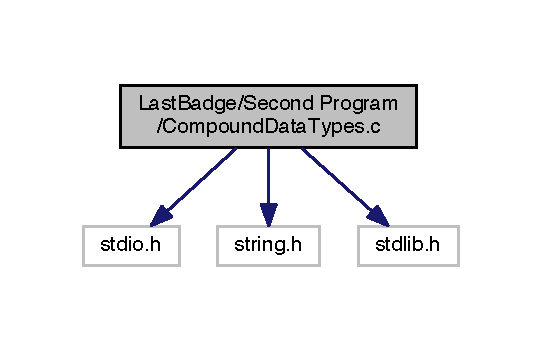
\includegraphics[width=260pt]{_compound_data_types_8c__incl}
\end{center}
\end{figure}
\subsection*{Data Structures}
\begin{DoxyCompactItemize}
\item 
struct \hyperlink{structmember}{member}
\end{DoxyCompactItemize}
\subsection*{Functions}
\begin{DoxyCompactItemize}
\item 
void \hyperlink{_compound_data_types_8c_ac824407a071ffa93870f9a28c4d7872a}{change} (struct \hyperlink{structmember}{member} $\ast$user)
\item 
int \hyperlink{_compound_data_types_8c_ae66f6b31b5ad750f1fe042a706a4e3d4}{main} ()
\end{DoxyCompactItemize}


\subsection{Function Documentation}
\hypertarget{_compound_data_types_8c_ac824407a071ffa93870f9a28c4d7872a}{\index{Compound\+Data\+Types.\+c@{Compound\+Data\+Types.\+c}!change@{change}}
\index{change@{change}!Compound\+Data\+Types.\+c@{Compound\+Data\+Types.\+c}}
\subsubsection[{change}]{\setlength{\rightskip}{0pt plus 5cm}void change (
\begin{DoxyParamCaption}
\item[{struct {\bf member} $\ast$}]{user}
\end{DoxyParamCaption}
)}}\label{_compound_data_types_8c_ac824407a071ffa93870f9a28c4d7872a}


 Module Name\+: change

Original Author\+: Nishant Jain

Module Creation Date\+: December 6, 2014

Description\+: This function allows user to change struct values

Required Files/\+Databases\+: None

Non System Routines Called\+: None

Return Value\+: None

O\+S Specific Assumptions\+: None

Local Variables\+: choice char-\/array Used to take input for user's choice sub int Subject score to change 

Definition at line 194 of file Compound\+Data\+Types.\+c.



Here is the caller graph for this function\+:\nopagebreak
\begin{figure}[H]
\begin{center}
\leavevmode
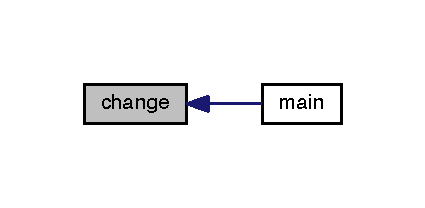
\includegraphics[width=204pt]{_compound_data_types_8c_ac824407a071ffa93870f9a28c4d7872a_icgraph}
\end{center}
\end{figure}


\hypertarget{_compound_data_types_8c_ae66f6b31b5ad750f1fe042a706a4e3d4}{\index{Compound\+Data\+Types.\+c@{Compound\+Data\+Types.\+c}!main@{main}}
\index{main@{main}!Compound\+Data\+Types.\+c@{Compound\+Data\+Types.\+c}}
\subsubsection[{main}]{\setlength{\rightskip}{0pt plus 5cm}int main (
\begin{DoxyParamCaption}
{}
\end{DoxyParamCaption}
)}}\label{_compound_data_types_8c_ae66f6b31b5ad750f1fe042a706a4e3d4}


 Module Name\+: main

Original Author\+: Nishant

Module Creation Date\+: December 5, 2014

Description\+: Inputs user information into a struct and calls \hyperlink{_compound_data_types_8c_ac824407a071ffa93870f9a28c4d7872a}{change()}

Required Files/\+Databases\+: None

Non System Routines Called\+: None

Return Value\+: Type Description int return(0)

O\+S Specific Assumptions\+: None

Local Variables\+: Name Type Description user struct member Data structure stores user's information ch char User's choice of operation k int Used to put initials of user's name in the string length int Length of string storing user's name Per float Percentage of user's marks Flowchart\+: 

Allocating memory to user name using callpc. Initiallizing it with N\+U\+L\+L

Reallocating more memory to name

Passing a pointer to function as parameter Call by reference

Allocating memory to length using malloc()

Freeing allocated memory 

Definition at line 62 of file Compound\+Data\+Types.\+c.



Here is the call graph for this function\+:\nopagebreak
\begin{figure}[H]
\begin{center}
\leavevmode
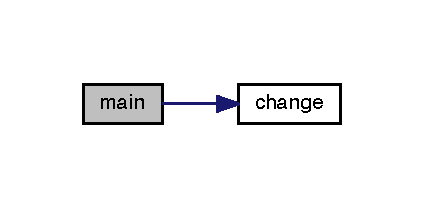
\includegraphics[width=204pt]{_compound_data_types_8c_ae66f6b31b5ad750f1fe042a706a4e3d4_cgraph}
\end{center}
\end{figure}



%--- End generated contents ---

% Index
\newpage
\phantomsection
\addcontentsline{toc}{chapter}{Index}
\printindex

\end{document}
